\newpage
\subsection{Лабораторная работа №2. Триггеры}

Задачи к лабораторной работе №2:

\begin{enumerate}
\item создать таблицу для хранения сводной информации о количестве поселений и платежей каждого студента; 
\item реализовать триггеры для автоматического изменения сводной информации при добавлении, изменении и удалении записей в таблицах \texttt{student}, \texttt{settlement} и \texttt{payment}; 
\item проверить корректность работы триггеров и автоматическое обновление сводной таблицы при изменении связанных данных.
\end{enumerate}

\subsubsection{Создание сводной таблицы}

Для хранения сводной информации о количестве поселений и платежей каждого студента была создана таблица
\texttt{student\_settlement\_payment\_counts}.

Таблица содержит идентификатор студента, его фамилию, имя и отчество, а также количество связанных с ним поселений и платежей. Первоначальное заполнение таблицы выполняется на основе уже существующих записей таблиц \texttt{student}, \texttt{settlement} и \texttt{payment}.

Для подсчёта количества поселений используется таблица \texttt{settlement}, а для подсчёта количества платежей --- таблица \texttt{payment}. Связь между студентом и платежом осуществляется через таблицу \texttt{settlement}.

Код создания и первоначального заполнения сводной таблицы представлен в листинге~\ref{lst:student_settlement_payment_counts}.

\begin{lstlisting}[
    language=SQL,
    caption={Создание таблицы student\_settlement\_payment\_counts},
    label={lst:student_settlement_payment_counts}
]
CREATE TABLE student_settlement_payment_counts AS
SELECT
    student.student_id,
    student.last_name,
    student.first_name,
    student.middle_name,
    COUNT(DISTINCT settlement.settlement_id) AS settlement_count,
    COUNT(DISTINCT payment.payment_id) AS payment_count
FROM
    student
    LEFT JOIN settlement
        ON student.student_id = settlement.student_id
    LEFT JOIN payment
        ON settlement.settlement_id = payment.settlement_id
GROUP BY
    student.student_id,
    student.last_name,
    student.first_name,
    student.middle_name;
\end{lstlisting}

Для обеспечения уникальности записей по каждому студенту столбец \texttt{student\_id} был определён в качестве первичного ключа. Код создания первичного ключа представлен в листинге~\ref{lst:primary_key}.

\begin{lstlisting}[
    language=SQL,
    caption={Создание первичного ключа таблицы student\_settlement\_payment\_counts},
    label={lst:primary_key}
]
ALTER TABLE student_settlement_payment_counts
ADD PRIMARY KEY (student_id);
\end{lstlisting}

Таким образом, в таблице \texttt{student\_settlement\_payment\_counts} для каждого студента хранится одна запись со следующими значениями:

\begin{itemize}
    \item \texttt{student\_id} --- идентификатор студента;
    \item \texttt{last\_name} --- фамилия студента;
    \item \texttt{first\_name} --- имя студента;
    \item \texttt{middle\_name} --- отчество студента;
    \item \texttt{settlement\_count} --- количество поселений;
    \item \texttt{payment\_count} --- количество платежей.
\end{itemize}

Схема базы данных после создания сводной таблицы представлена на рисунке~\ref{fig:student_settlement_payment_counts}.

\subsubsection{Создание триггеров}

После создания и первоначального заполнения сводной таблицы были реализованы триггеры, предназначенные для автоматического поддержания актуальности значений \texttt{settlement\_count} и \texttt{payment\_count}.

Триггеры создаются для таблиц \texttt{student}, \texttt{settlement} и \texttt{payment}. Все реализованные триггеры являются триггерами типа \texttt{AFTER} и выполняются для каждой изменённой строки с использованием конструкции \texttt{FOR EACH ROW}.

\subsubsection{Триггер таблицы student}

Для таблицы \texttt{student} был создан триггер \texttt{after\_student\_delete}, срабатывающий после удаления записи.

При удалении студента соответствующая запись должна быть удалена и из сводной таблицы
\texttt{student\_settlement\_payment\_counts}. Для поиска записи используется идентификатор удалённого студента \texttt{OLD.student\_id}.

Код триггера представлен в листинге~\ref{lst:student_triggers}.

\begin{lstlisting}[
    language=SQL,
    caption={Триггер удаления студента},
    label={lst:student_triggers}
]
CREATE OR REPLACE FUNCTION after_student_delete()
RETURNS TRIGGER
AS $$
BEGIN
    DELETE FROM student_settlement_payment_counts
    WHERE student_id = OLD.student_id;

    RETURN OLD;
END;
$$ LANGUAGE plpgsql;

CREATE TRIGGER after_student_delete
AFTER DELETE ON student
FOR EACH ROW
EXECUTE FUNCTION after_student_delete();
\end{lstlisting}

Таким образом, при удалении студента автоматически удаляется соответствующая запись из сводной таблицы. Это предотвращает появление в сводной таблице записей о студентах, отсутствующих в таблице \texttt{student}.

\subsubsection{Триггеры таблицы settlement}

Для таблицы \texttt{settlement} были созданы триггеры для операций добавления, удаления и изменения записей.

Триггер \texttt{after\_settlement\_insert} срабатывает после добавления нового поселения. Для соответствующего студента значение \texttt{settlement\_count} увеличивается на единицу.

Триггер \texttt{after\_settlement\_delete} срабатывает после удаления поселения. Для студента, которому принадлежало удалённое поселение, значение \texttt{settlement\_count} уменьшается на единицу.

Триггер \texttt{after\_settlement\_update} срабатывает после изменения записи поселения. Если поселение было связано с другим студентом, количество поселений у предыдущего студента уменьшается на единицу, а у нового студента увеличивается на единицу.

Код триггеров представлен в листинге~\ref{lst:settlement_triggers}.

\begin{lstlisting}[
    language=SQL,
    caption={Триггеры для таблицы settlement},
    label={lst:settlement_triggers}
]
CREATE OR REPLACE FUNCTION after_settlement_insert()
RETURNS TRIGGER
AS $$
BEGIN
    UPDATE student_settlement_payment_counts
    SET settlement_count = settlement_count + 1
    WHERE student_id = NEW.student_id;

    RETURN NEW;
END;
$$ LANGUAGE plpgsql;

CREATE TRIGGER after_settlement_insert
AFTER INSERT ON settlement
FOR EACH ROW
EXECUTE FUNCTION after_settlement_insert();


CREATE OR REPLACE FUNCTION after_settlement_delete()
RETURNS TRIGGER
AS $$
BEGIN
    UPDATE student_settlement_payment_counts
    SET settlement_count = settlement_count - 1
    WHERE student_id = OLD.student_id;

    RETURN OLD;
END;
$$ LANGUAGE plpgsql;

CREATE TRIGGER after_settlement_delete
AFTER DELETE ON settlement
FOR EACH ROW
EXECUTE FUNCTION after_settlement_delete();


CREATE OR REPLACE FUNCTION after_settlement_update()
RETURNS TRIGGER
AS $$
BEGIN
    IF OLD.student_id IS NOT NULL THEN
        UPDATE student_settlement_payment_counts
        SET settlement_count = settlement_count - 1
        WHERE student_id = OLD.student_id;
    END IF;

    IF NEW.student_id IS NOT NULL THEN
        UPDATE student_settlement_payment_counts
        SET settlement_count = settlement_count + 1
        WHERE student_id = NEW.student_id;
    END IF;

    RETURN NEW;
END;
$$ LANGUAGE plpgsql;

CREATE TRIGGER after_settlement_update
AFTER UPDATE ON settlement
FOR EACH ROW
EXECUTE FUNCTION after_settlement_update();
\end{lstlisting}

\subsubsection{Триггеры таблицы payment}

Для таблицы \texttt{payment} также были созданы триггеры для операций добавления, удаления и изменения записей.

Таблица \texttt{payment} не содержит непосредственной связи со студентом. Связь с ним осуществляется через таблицу \texttt{settlement}: каждая запись о платеже содержит идентификатор поселения \texttt{settlement\_id}, по которому определяется соответствующий \texttt{student\_id}.

Триггер \texttt{after\_payment\_insert} срабатывает после добавления платежа и увеличивает значение \texttt{payment\_count} для студента, которому принадлежит соответствующее поселение.

Триггер \texttt{after\_payment\_delete} срабатывает после удаления платежа и уменьшает значение \texttt{payment\_count} для соответствующего студента.

Триггер \texttt{after\_payment\_update} срабатывает после изменения платежа. Если изменяется поселение, с которым связан платеж, количество платежей у студента старого поселения уменьшается на единицу, а у студента нового поселения увеличивается на единицу.

Код триггеров представлен в листинге~\ref{lst:payment_triggers}.

\begin{lstlisting}[
    language=SQL,
    caption={Триггеры для таблицы payment},
    label={lst:payment_triggers}
]
CREATE OR REPLACE FUNCTION after_payment_insert()
RETURNS TRIGGER
AS $function$
BEGIN
    UPDATE student_settlement_payment_counts
    SET payment_count = payment_count + 1
    WHERE student_id = (
        SELECT student_id
        FROM settlement
        WHERE settlement_id = NEW.settlement_id
    );

    RETURN NEW;
END;
$function$ LANGUAGE plpgsql;

CREATE TRIGGER after_payment_insert
AFTER INSERT ON payment
FOR EACH ROW
EXECUTE FUNCTION after_payment_insert();


CREATE OR REPLACE FUNCTION after_payment_delete()
RETURNS TRIGGER
AS $function$
BEGIN
    UPDATE student_settlement_payment_counts
    SET payment_count = payment_count - 1
    WHERE student_id = (
        SELECT student_id
        FROM settlement
        WHERE settlement_id = OLD.settlement_id
    );

    RETURN OLD;
END;
$function$ LANGUAGE plpgsql;

CREATE TRIGGER after_payment_delete
AFTER DELETE ON payment
FOR EACH ROW
EXECUTE FUNCTION after_payment_delete();


CREATE OR REPLACE FUNCTION after_payment_update()
RETURNS TRIGGER
AS $function$
BEGIN
    IF OLD.settlement_id IS NOT NULL THEN
        UPDATE student_settlement_payment_counts
        SET payment_count = payment_count - 1
        WHERE student_id = (
            SELECT student_id
            FROM settlement
            WHERE settlement_id = OLD.settlement_id
        );
    END IF;

    IF NEW.settlement_id IS NOT NULL THEN
        UPDATE student_settlement_payment_counts
        SET payment_count = payment_count + 1
        WHERE student_id = (
            SELECT student_id
            FROM settlement
            WHERE settlement_id = NEW.settlement_id
        );
    END IF;

    RETURN NEW;
END;
$function$ LANGUAGE plpgsql;

CREATE TRIGGER after_payment_update
AFTER UPDATE ON payment
FOR EACH ROW
EXECUTE FUNCTION after_payment_update();
\end{lstlisting}

\subsubsection{Проверка работы триггеров}

Для проверки корректности работы созданных триггеров были выполнены операции добавления, удаления и изменения записей в таблицах \texttt{student}, \texttt{settlement} и \texttt{payment}. После каждой операции проверялось автоматическое изменение соответствующей записи в таблице
\texttt{student\_settlement\_payment\_counts}.

При добавлении нового поселения значение \texttt{settlement\_count} соответствующего студента увеличивается на единицу. При удалении поселения это значение уменьшается на единицу.

При изменении студента, которому принадлежит поселение, значение \texttt{settlement\_count} уменьшается для прежнего студента и увеличивается для нового.

Аналогичным образом проверяется работа триггеров для таблицы \texttt{payment}. После добавления платежа значение \texttt{payment\_count} соответствующего студента увеличивается на единицу, а после удаления платежа --- уменьшается на единицу.

При изменении \texttt{settlement\_id} платежа производится корректировка счётчиков у студентов, связанных со старым и новым поселениями.

Также была проверена обработка удаления студента. После удаления записи из таблицы \texttt{student} соответствующая запись автоматически удаляется из таблицы
\texttt{student\_settlement\_payment\_counts}.

Таким образом, результаты проверки показывают, что созданные триггеры автоматически поддерживают значения \texttt{settlement\_count} и \texttt{payment\_count} в соответствии с изменениями связанных таблиц.

\begin{table}[H]
\centering
\caption{Действия созданных триггеров}
\label{tab:trigger_actions}
\begin{tabularx}{\textwidth}{|c|X|}
\hline
\textbf{№} & \textbf{Действие} \\ \hline

1 &
Удаление студента из таблицы \texttt{student}. В таблице
\texttt{student\_settlement\_payment\_counts} удаляется
соответствующая запись.
\\ \hline

2 &
Добавление поселения в таблицу \texttt{settlement}. Счётчик
поселений для указанного студента увеличивается на 1.
\\ \hline

3 &
Удаление поселения из таблицы \texttt{settlement}. Счётчик
поселений для указанного студента уменьшается на 1.
\\ \hline

4 &
Изменение студента у поселения в таблице \texttt{settlement}.
Счётчик для нового студента увеличивается на 1, а для старого
уменьшается на 1.
\\ \hline

5 &
Добавление платежа в таблицу \texttt{payment}. Счётчик платежей
для соответствующего студента увеличивается на 1.
\\ \hline

6 &
Удаление платежа из таблицы \texttt{payment}. Счётчик платежей
для соответствующего студента уменьшается на 1.
\\ \hline

7 &
Изменение поселения у платежа в таблице \texttt{payment}.
Счётчик для студента нового поселения увеличивается на 1,
а для старого уменьшается на 1.
\\ \hline

\end{tabularx}
\end{table}

\clearpage
\begin{landscape}
    \thispagestyle{empty}
   \begin{figure}[H]
    \centering
    \vfill
    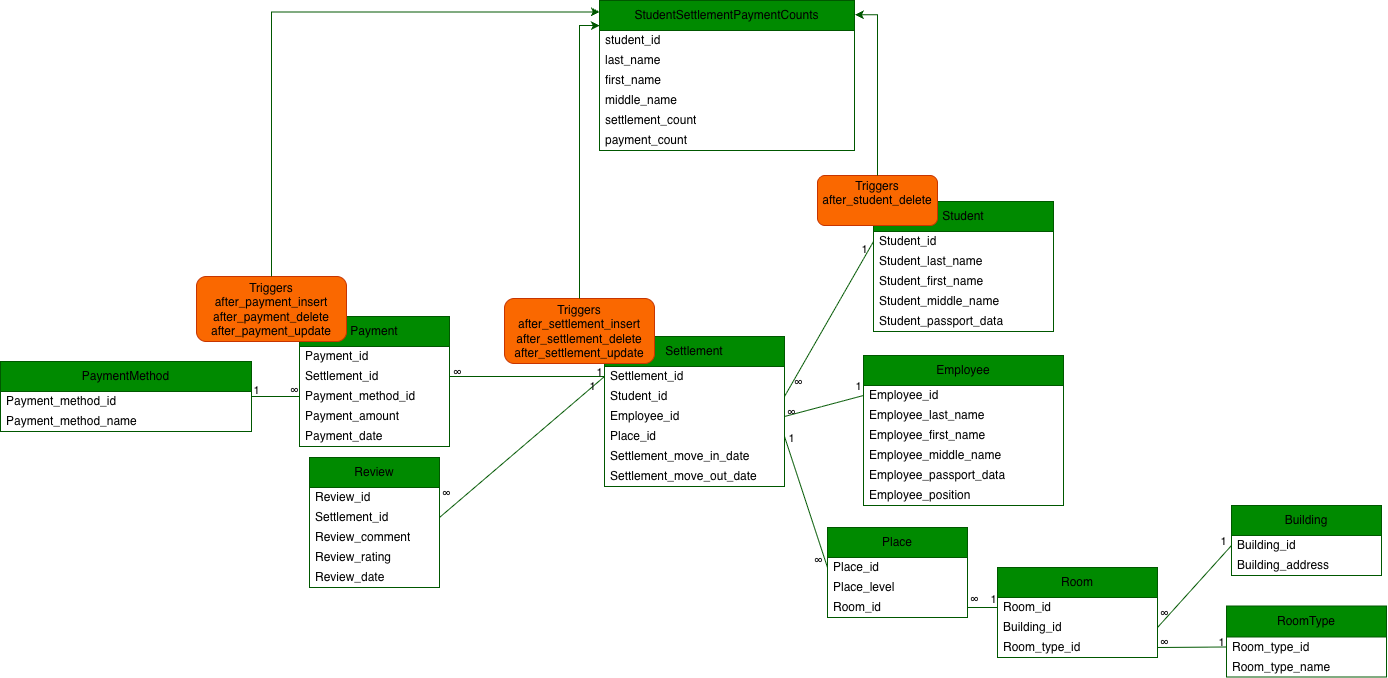
\includegraphics[width=\linewidth]{figures/db-schema-en.png}
    \caption{Графическое представление создания представления}
    \label{fig:student_settlement_payment_counts}
    \vfill
\end{figure}
\end{landscape}
\clearpage
